\section{\SemiEmpirical Theory of the \HTSR Phenomenology}
\label{sxn:matgen}

In this section, we present the main technical elements of our \SemiEmpirical Theory of Deep Learning (\SETOL).
Our goal is to explain and, where possible, derive the \HTSR PL metrics \ALPHA $(\alpha)$ and \ALPHAHAT $\hat{\alpha}$
from first principles, and, in doing so, also present the \TRACELOG condition and
newly proposed \WW\DETX metric.
To do this, we introduce a Matrix Generalization of the Student-Teacher model for a Linear \Perceptron
(See Section~\ref{sxn:SMOG_main-st_av}), 
adapted here for a (3-layer) \MultiLayerPerceptron  (MLP3).
We seek a theory for the \LayerQuality $\Q=\Q^{NN}_{L}$ of a NN, where
this \LayerQuality now corresponds to the (approximate) contribution each layer makes to the total
generalization accuracy, or total \Quality $\Q^{NN}$.
For technical reasons, we actually seek a formal expression(s) for the \LayerQualitySquared,
$\QT\approx\Q^{2}$. 
We say that the \SETOL is \SemiEmpirical because the final result $\QT$ is expressed directly in terms
of the empirically observable spectral properties of the Teacher layer weight matrix $\TMAT=\WMAT$.


%\red{REMOVED OUTLINE REPACE WITH SECTION 5.1: need to rework the paragraph above and below, merge}
%\paragraph{Outline}
%\begin{itemize}
%\item In Section~\ref{sxn:matgen_basic_elements}, we provide an overview of basic elements of our approach.
%
%\item In Section~\ref{sxn:matgen_mlp3}, we describe the matrix generalization of the ST  model of the \LinearPerceptron.
%
%\item In Section~\ref{sxn:matgen_quality_hciz}, we describe how to generalize the (Thermal) average over the Students to an integral over random \Student matrices, called an HCIZ integral.
%
%\item In Section~\ref{sxn:matgen_evaluation_hciz}, we describe how to evaluate the HCIZ integral in the large-$N$ limit.
%
%\item In Section~\ref{sxn:r_transforms}, we explain how to select an \RTransform and evaluate the \michael{such-and-such-not-sure-if-we-should-call-it-norm-gf} under different modeling assumptions.
%\end{itemize}

%\subsection{Basic Elements of the \SemiEmpirical Theory}
%\label{sxn:matgen_basic_elements_concise}

\begin{enumerate}[label=5.\arabic*]
\item
\textbf{Matrix Generalization of the ST Model.}
Section~\ref{sxn:matgen_mlp3} generalizes
classical \STATMECH vector-based ST model of Section~\ref{sxn:SMOG_main-student_teacher}
to obtain a \LayerQuality for a single layer in a NN.
It starts by first formulating the learning problem for
the NN generalization accuracy or quality, $\Q^{NN}$,
of a 3-layer MLP (MLP3).
We then replace vectors with $N \times M$ matrices $\SVEC,\TVEC\rightarrow\SMAT,\TMAT$,
and obtain and expression for the NN \SelfOverlap $\ETA(\SMAT,\TMAT,\XI)$,which then gives a matrix-generalized overlap operator
$\OVERLAP:=\langle\ETA(\SMAT,\TMAT,\XI)\rangle_{\AVGNDXI}=\tfrac{1}{N}\SMAT^{\top}\TMAT$.
This can be related to a single-layer matrix-generalization of the ST \AnnealedHamiltonian, 
presented in Appendix~\ref{sxn:summary_sst92},
$\HANHT:=\red{N}(M-\OVERLAP$),
where, importantly, the scalar overlap $R$ is now a matrix $\OVERLAP$ of $M\times M$ adjustable parameters.
\red{And, importantly, being empirical quantities, the matrices are implicitly normalized to $1/\ND$.}

\item
\textbf{The \LayerQualitySquared $\QT$.}
Section~\ref{sxn:matgen_quality_hciz} presents the expression for NN \LayerQualitySquared $\QT$.
Following the ST analogy, we define a \ThermalAverage over possible \Student weight matrices $\SMAT$
for the matrix overlap, giving $\Q^{NN}_{L}:=\THRMAVGIZ{\HANHT} =\THRMAVGIZ{\OVERLAP}$.
For technical reasons, however, we actually seek the (approximate)  \LayerQualitySquared, $\QT\approx (\Q^{NN}_{L})^2$,
defined as $\QT:=\THRMAVGIZ{\OLAPTOLAP}$.
To evaluate $\QT$, rather than sampling all random \Student matrices $\SMAT$ directly,
we switch measures to the (Outer) \Student Correlation matrices\footnote{
We adopt the convention ``Inner'' for smaller, $M\times M$ full rank \Student correlation matrices, and ``Outer'' for larger, $N\times N$ rank-deficient \Student Correlation matrices.
Note that both are scaled as $1 / N$, meaning that their nonzero eigenvalues are the same.
} 
$\AMATN = \tfrac{1}{N}\SMAT\SMAT^{\top}$ along with their Inner counterparts
$\AMATM = \tfrac{1}{N}\SMAT^{\top}\SMAT$.
Importantly, we argue that the measures $d\mu(\AMATM)\leftrightarrow d\mu(\AMATN)$,
can be interchanged for our purposes, making them effectively equivalent.
This reparameterization leads us to an integral of the HCIZ type (as in \EQN~\ref{eqn:hciz_prelim})
which, as shown by Tanaka \cite{Tanaka2007, Tanaka2008}, can be described in terms of its R-transform.

Then, we introduce the \EffectiveCorrelationSpace (\ECS), and two key approximations,
the \TRACELOG Condition and the \IndependentFluctuationApproximation (\IFA).
The \TRACELOG condition states that the determinant of the (effective) \Student correlation matrix is unity, $\Det{\AECS}=1$.
Critically, this condition can be tested empirically by assuming the (effective) \Teacher correlation matrix
also follows the \TRACELOG condition, $\Det{\XECS}=1$, and this is a key result of this work.
Finally, we impose the \IFA (described below) because it is necessary for the final result.

\item
\textbf{The \LargeN limit in $N$}
Section~\ref{sxn:matgen_evaluation_hciz} presents the core result,
(as in \EQN~\ref{eqn:QT_result}),
closed-form or semi-analytic expression(s) for the \LayerQualitySquared $\QT$
formed in the "wide" \largeN limit in $N$.
Restricted to the \ECS, and under the \TRACELOG condition and the \IFA, our
HCIZ integral for $\QT$ becomes tractable at large-$N$, giving an expression that can be parameterized
in terms of $\MECS$ eigenvalues $\LambdaECS$ of the \Teacher correlation matrix 
restricted to the \ECS $\XECS$.
In doing this, the $\MECS$ \Teacher eigenvalues are treated as experimental observables, and 
become the effective \SemiEmpirical parameters (i.e., $\alpha$, $\LambdaMax$) of our \SETOL.

\item
\textbf{Modeling the \HeavyTailed \RTransform}
Section~\ref{sxn:r_transforms} presents several models of different \RTransforms.
Evaluating $\QT$ requires evaluating selecting an \RTransform $R(z)$ for the Teacher Empirical Spectral Density (ESD),
and also ensure that it is analytic and single-valued on the domain of interest-- the \ECS and/or tail of the ESD.
We examine four possible models for $R(z)$: \emph{(i)} the \emph{Bulk$+$Spikes} (BS),
\emph{(ii)} the \emph{Free Cauchy} (FC) model, 
\emph{(iii)} the \emph{\InverseMP} (IMP) model, 
and \emph{(iv)} the  \LevyWigner (LW) model.
First, as a trivial case, the tail of ESD can be treated as a collection of spikes,
and the ESD is simply a sum of Dirac delta functions; in this case,
$\QT$ becomes a ``Tail Norm'', the Frobenius Norm of the PL tail.
When the layer is \Ideal, i.e., $\alpha\sim 2$ and $\Det{\XECS}\sim 1$,
one can use  \emph{Free Cauchy} (FC) model.  and the resulting \LayerQuality $\Q$
is approximately the Spectral Norm $\LambdaMax$.
Since $\LambdaMax$ increases with decreasing $\alpha$, the FC model yields the \HTSR \ALPHA metric.
One can also use  \emph{\InverseMP} (IMP) model. 
As required, the IMP \RTransform contains a \emph{branch cut} in the complex plane
which aligns with the start of the \ECS \PowerLaw tail.
Finally, Using the \LevyWigner (LW) model, one can model cases where
$\alpha\le 2$ and derive the \HTSR \ALPHAHAT metric.
\end{enumerate}

\vspace*{1em}

These core elements form a bridge between well-established empirical properties of large-scale NNs 
and a tractable ST-based theory. In the subsequent sections, we formalize the key steps: 
\emph{(i)} setting up the matrix-based ST problem, \emph{(ii)} defining our HCIZ integrals 
over restricted correlation matrices (\ECS), and \emph{(iii)} analyzing the resulting 
\emph{Layer Quality} (or \emph{Quality-Squared}) expressions in the large-$N$ limit.

\subsection{\MultiLayer Setup: MLP3}
\label{sxn:matgen_mlp3}

In this section, we describe the matrix generalization of the ST  model of the \LinearPerceptron; and, 
in particular, a matrix-generalized version of the key quantities we derived in Section~\ref{sxn:SMOG_main-st_av}.

\paragraph{A simple model.}

Consider a simple NN with three layers (two hidden and an output), i.e., a three-layer \MultiLayerPerceptron, denoted as the \emph{MLP3} model.
(This is a \emph{very} simple model of a modern NN with hundreds of layers and complex internal structure.)

Ignoring the bias terms, \emph{Without Loss of Generality}, (WLOG), the NN outputs
 $E_{1\mu},E_{2\mu},E_{3\mu}$ for each layer, as defined in \EQN~\ref{eqn:dnn_energy}, are given by:
\begin{align}
\nonumber
  E_{1\mu} &:= \frac{1}{\sqrt{N_1}} h (\mathbf{W}_1^\top \boldsymbol{\xi}_{\mu}) , \\
\nonumber
  E_{2\mu} &:= \frac{1}{\sqrt{N_2}} h (\mathbf{W}_2^\top \mathbf{Z}_{1\mu})     , \\
\label{eqn:nflow}
             y_{\mu} := E_{3\mu} &= \frac{1}{\sqrt{N_3}} h (\mathbf{W}_{3}^\top \mathbf{Z}_{2\mu})     ,
\end{align}
where $h$ is a general function or functional, denoting either a non-linear activation or a more complex layer structure, such as a CNN or an RNN.
We can consider $h(\cdot)$ to be an (unspecified) activation function.

Let us specify the ST error, or Energy difference, specifically in terms of the L2 or RMSE loss:
\begin{equation}
\label{eqn:DE}
\DETOPNN = \frac{1}{2}\sum_{\mu=1}^{\ND} (\Ys - \Yt)^2.
\end{equation}

We now start to develop the self-overlap \(\eta\) using \(\mathbf{S} - \mathbf{T}\):

\subsubsection{Data-Dependent Multi-Layer ST Self-Overlap $(\ETA(\SMAT,\TMAT))$}

It is convenient to rewrite $\Delta \mathbf{\hat{E}}$ in \EQN~\ref{eqn:DE} as:
\begin{align}
\label{eqn:DE2}
\DETOPNN
   := \frac{1}{2} \Trace{ (\Ys - \Yt)^\top (\Ys - \Yt) }
   = N - \Trace{ (\YsVEC)^{\top} \, \YtVEC  }
   = N(1 - \ETAMLPXI)
\end{align}
where the \SelfOverlap $\ETAMLPXI$
is of the same form as the (vector) \LinearPerceptron (in \EQN~\ref{eqn:deriveSTerror}).
Note that $\ETAMLPXI$ depends on the (model) data $\boldsymbol{\xi}$
because we have not evaluated the expected value $\langle \cdots \rangle_{\boldsymbol{\xi}}$ yet.

Using the general expression from \EQN~\ref{eqn:nflow} for the action of the NN on the input data $\boldsymbol{\xi}$,
we can write the formal expression of the ST error for the simple MLP3 model as:
\begin{align}
\label{eqn:overlap1}
\ETAMLPAVG  \\ \nonumber
& =\langle\ETA(\SMAT_1,\SMAT_2,\SMAT_3,\TMAT_1,\TMAT_2,\TMAT_3,\boldsymbol{\xi})\rangle_{\AVGNDXI}  \\ \nonumber
& :=  \Trace{
    \frac{1}{\sqrt{N_3}} h\left(\mathbf{S}_3^{\top} 
    \frac{1}{\sqrt{N_2}} h\left(\mathbf{S}_2^{\top} 
    \frac{1}{\sqrt{N_1}} h\left(\mathbf{S}_1^{\top} \boldsymbol{\xi} \right)\right)\right)^{\top} 
    \times
    \frac{1}{\sqrt{N_3}} h\left(\mathbf{T}_3^{\top} 
    \frac{1}{\sqrt{N_2}} h\left(\mathbf{T}_2^{\top} 
    \frac{1}{\sqrt{N_1}} h\left(\mathbf{T}_1^{\top} \boldsymbol{\xi} \right)\right)\right)
  }.
\end{align}

So far, we have not used any particular assumption on the form of the NN or the data, 
\michael{But this is the model Gaussian data, not the real data}
\charles{Yeah, I guess thats in the notation, but we have not integrated out the data yet.  We can rephrase this}
other than that the layer structure used to write the explicit expression for the form eventually xneeded,
$\ETA(\SMAT,\TMAT)$, a single layer \SelfOverlap.
As a next step, we show which assumptions are needed in order to reformulate the setup as
an effectively a single layer linear model for a NN.

\michael{The following change to single layer holds for L2 and non-L2, correct?  If so, why mention L2 in \EQN~\ref{eqn:DE} and \EQN~\ref{eqn:DE2}, and then go back to more general in \EQN~\ref{eqn:overlap1}.}
\charles{um no I think the square is necessary }

\subsubsection{A Single Layer Matrix Model}

Following others in the literature~\cite{SMG2013_TR}, and for simplicity, one can restrict to the simplifying case that the function $h(x)$ is the identity function.
To evaluate \EQN~\ref{eqn:overlap1}, there are three possibilities.
First, we can multiply all the matrices together, and treat a multi-layer NN effectively as a single layer.
Under this assumption, \EQN \ref{eqn:overlap1} simplifies to
%
\begin{align}
\label{eqn:overlap2}
  \ETAMLPAVG &= \tfrac{1}{N_3 \, N_2 \, N_1} 
  \Trace{ \boldsymbol{\xi}^\top 
    \mathbf{S}_1 \mathbf{S}_2 \mathbf{S}_3 
    \mathbf{T}_3^{\top} \mathbf{T}_2^{\top} \mathbf{T}_1^{\top} 
    \boldsymbol{\xi} }.
\end{align}
While this is possible, it would not lead to layer-by-layer insights (as \HTSR-based approaches do).
%
Second, we could attempt to expand \EQN~\ref{eqn:overlap2} into inter- and intra-layer terms, 
which we could readily do if the $S$ and $T$ matrices were square and the same shape, and then apply Wicks theorem:
\begin{align}
\ETAMLP\approx\prod_{l=1}^{L}\tfrac{1}{N_l}\ETAMATAVG=\prod_{l=1}^{L}\tfrac{1}{N_l}\Trace{ \XI^{\top} \mathbf{S}^{\top}_{l} \mathbf{T}_{l} \XI) } +\text{intra-layer cross terms}.
\end{align}
However, these matrices are not square, and we don't know how to express the intra-layer cross terms.
%
Finally, we can simply assume that the individual layers are statistically independent, in which case we can treat each layer independently.
By ignoring the intra-layer cross-terms, let us write the single-layer self-overlap $\ETAMAT$ as:
\begin{align}
  \label{eqn:eta}
  \ETAMAT =
        \ETAMATAVG\rightarrow \tfrac{1}{N} \Trace{ \XI^{\top} \mathbf{S}^{\top}_{l} \mathbf{T}_{l} \XI }  .
\end{align}
This third approach is the one we will adopt.
Moving forward, we will drop the layer subscript, $l$, and we will consider a \SETOL as a single-layer theory.


\subsubsection{The Matrix-Generalized ST Overlap $(\ETA(\SMAT,\TMAT)$)}

We can now relate the \SelfOverlap for the NN layer $\ETA(\XI)_{l}$ in \EQN~\ref{eqn:eta}
as a matrix-generalized form of the ST \EffectivePotential $\EPSL(R)=1-R$.
\michaeladdressed{We are calling it \EffectivePotential there; not sure if we are going to use that term or the other, consistently throughout.}
Since we can interpret the Trace as an expected value over the model data $\NDXI$, this gives the desired
\begin{align}
  \label{eqn:eta_mat_avg_def}
  \ETA(\SMAT,\TMAT)
  :=\tfrac{1}{N} \Trace{\mathbf{S}^{\top}\mathbf{T}} 
\end{align}
This is the matrix generalized form of \EQN~\ref{eqn:QST_final} for the \LayerQuality.


\subsection{Quality Metrics of an Individual Layer as an HCIZ Integral}
\label{sxn:matgen_quality_hciz}

In this subsection, we describe how to generalize the (Thermal) average over the Students $\THRMAVG{\cdots}$ to an 
integral over random \Student matrices, $\THRMAVGIZ{\cdots}$, called an HCIZ integral.

\subsubsection{A Generating Function Approach to Average \QualitySquared of a Layer}
\label{sxn:matgen_quality_hciz_A}

For our matrix generalization, we need to express the \LayerQuality $\Q$ in terms of the data-averaged
\SelfOverlap in \EQN~\ref{eqn:eta_mat_avg_def} for a individual layer.
\begin{itemize}
\item
\textbf{Student-Teacher Overlap  $\mathbf{R}$}
For the vector-based \Perceptron ST model, the data-averaged \SelfOverlap appears in the expression for the
\LayerQuality  in \EQN~\ref{eqn:QST_final}, and is just the average ST vector overlap $R=\SVEC^{\top}\TVEC$. 
We define 
\begin{equation}
\mathbf{R} =  \frac{1}{N}\SMAT^{T} \TMAT  .
\end{equation}
The overlap matrix $\OVERLAP$ describes the average interactions between $N$ interacting $M$-dimensional layer (i.e., feature) vectors.  Also, notice that we have dropped $1/\ND$ term.
For the vector-based ST model, the ST \Quality $\Q^{ST}$ in \EQN~\ref{eqn:QST_final} is expressed as
the \ThermalAverage $\Q^{ST}(\AVGR)=\THRMAVG{\AVGR}$. We seek a similar formal expression for the individual matrx-generalized \LayerQuality $\Q^{NN}_{L}$.
\item
\textbf{Model and Layer Qualities $\Q^{NN}$, $\Q^{NN}_{L}$}
We define the \ModelQuality $\Q^{NN}$ ,
as explained in Subsection~\ref{sxn:htsr-metics}, \EQN~\ref{eqn:ProductNorm},
to be a product of individual NN Layer Qualities $\Q^{NN}_{L}$,
and, as in \EQN~\ref{eqn:model_qualities},
approximates the total NN \AverageGeneralizationAccuracy $(1-\AVGGE^{NN})$:
\begin{equation}
 \Q^{NN}:=\prod_{L}\Q^{NN}_{L}\approx 1-\AVGGE^{NN} 
\end{equation}
The individual $\Q^{NN}_{L}$ expresses the contribution that layer makes
to the approximate total NN \AverageGeneralizationAccuracy.
\item
 \textbf{\LayerQualitySquared $\QT$}
For  technical convenience, however, rather than compute
the NN \LayerQuality $\Q^{NN}_{L}$ directly, we will work with the \emph{\AverageLayerQualitySquared}, 
defined as
\begin{align}
  \label{eqn:QT_1}
  \QT:=\THRMAVGIZ{\OLAPTOLAP}
\end{align}
where  $\THRMAVGIZ{\cdots}$ is now a \ThermalAverage over Student weight matrices $\SMAT$--
an HCIZ integral.

This choice means that final \LayerQuality $\Q$ we use approximates what would be the
matrix-generalized NN \LayerQuality $\Q^{NN}_{L}$ (above) as
\begin{align}
  \label{eqn:QT_2}
  \Q:=\sqrt{\QT}
  =\sqrt{\THRMAVGIZ{\OLAPTOLAP}} \\ \nonumber
  \approx\THRMAVGIZ{\sqrt{\OLAPTOLAP}} \\ \nonumber
  \approx\THRMAVGIZ{\OVERLAP} \\ \nonumber
  = \Q^{NN}_{L}
\end{align}

\item
 \textbf{Overlap Squared}
 The Overlap operator (squared)  $\OLAPSQD$ is defined  in terms of \EQN~\ref{eqn:A2} such
 that we can 
\begin{align}
  \label{eqn:TraceR2withA2}
  \QT :=\OLAPSQD
  =\frac{1}{N^{2}}\Trace{\TMAT^{\top}\SMAT\SMAT^{\top}\TMAT}
  =\frac{1}{N}\Trace{\TMAT^{\top}\AMATN\TMAT}  .
\end{align}
This choice, (as opposed to $\Trace{\OVERLAP\OVERLAP^{\top}}$, which would correspond with \EQN~\ref{eqn:A1},) places $\QT$ in the form of the HCIZ integral, as in \EQN~\ref{eqn:hciz_prelim}.
See Appendix~\ref{sxn:tanaka} for a detailed discussion of why we define $\QT$ using the \emph{Outer} Student Correlation matrix $\AMATN$ (defined in Section~\ref{sxn:setol}, and  \EQN~\ref{eqn:A2} below).
\item
 \textbf{\GeneratingFunction}
For the vector-based ST model, we could compute $\Q^{ST}$ using a generating function, $\STG$.
For our matrix generalization, we compute $\Q$ from a \emph{\LayerQualitySquared \GeneratingFunction} $\IZG$, given as
\begin{align}
  \label{eqn:betaIZG_S}
  \IZG:=  \red{\tfrac{1}{N}}\ln \int d\mu(\SMAT) \exp\left[\ND\beta N\OLAPSQD\right] .
\end{align}
We normalize the $\IZG$ because we are going to take the \LargeN limit in $N$, and we need to keep the \LayerQuality finite.  This allows us to implicitly fix the effective load of the layer, $\ND/N$, as $\IZG$ is also in the \ThermodynamicLimit and therefore at \LargeN in $\ND$, although we do not explicitly set $\ND/N$.
See Appendix~\ref{sxn:quality} for the derivation of \EQN~\ref{eqn:betaIZG_S} (and recall the discussion in Section~\ref{sxn:mathP}). 
\end{itemize}

We cannot evaluate \EQN~\ref{eqn:betaIZG_S} directly; but we will be able to evaluate it if we transform it into an HCIZ integral (as in \EQN~\ref{eqn:hciz_prelim}). To do this, however, requires a trick which will allow us to work with different forms of the Student $\AMAT$ (and Teacher $\XMAT$) Correlation matrices.

\paragraph{From weight matrices to Correlation matrices.}
To evaluate $\QT$ in terms of derivatives of \EQN~\ref{eqn:betaIZG_S}, we need to introduce the change of measure:
\begin{align}
  \label{eqn:changeOfMeasure}
  d\mu(\SMAT)\rightarrow d\mu(\AMAT) ,
\end{align}
and then restrict $d\mu(\AMAT)$ to resemble just the generalizing eigencomponents of the \Teacher correlation matrix $\XMAT$.
%
%MM%
%MM%We now introduce the change of measure
%MM%\begin{align}
%MM%  \label{eqn:changeOfMeasure}
%MM%  d\mu(\SMAT)\rightarrow d\mu(\AMAT)
%MM%\end{align}
%MM%So before we evaluate $\QT$, we need to do this change of measure,
%MM%and do so that we restrict $d\mu(\AMAT)$ to resemble the just the
%MM%generalizing eigen-components of the \Teacher correlation matrix $\XMAT$.
%MM%
%\paragraph{Two choices for $\AMAT$}
We have two choices for the \Student \CorrelationMatrix $\AMAT$, call them $\AMATM$
(Inner) and $\AMATN$ (Outer), defined as:
\begin{eqnarray}
  \label{eqn:A1}
 \textrm{(Inner) }\;\AMATM&:=& \frac{1}{N}\SMAT^{\top}\SMAT \quad\mbox{(which is $M \times M$)} \\
  \label{eqn:A2}
 \textrm{(Outer) }\;\AMATN &:=& \frac{1}{N}\SMAT\SMAT^{\top} \quad\mbox{(which is $N \times N$)} .
\end{eqnarray}
Note that $\frac{1}{N}$ is the correct scaling on each of these.
\EQN~\ref{eqn:A1} is consistent with our definition of the layer \CorrelationMatrix, and we use it as the starting point
below to derive the \VolumePreserving \TRACELOG condition (Appendix~\ref{sxn:TraceLogDerivation}).
\EQN~\ref{eqn:A2} is consistent with Tanaka, which requires $\AMAT$ be $N\times N$, but
we still need a \emph{Duality of Measures} to rederive this (Appendix~\ref{sxn:tanaka})~\cite{Tanaka2007, Tanaka2008}.

\paragraph{Duality of measures.}
For either form of $\AMAT$, the measure $d\mu(\AMAT)$ is the same because we will restrict the measures to the~\ECS
space of non-zero eigenvalues $(\lambda_{i}\gg 0)$.
We note that $\AMATM$ and $\AMATN$ have the same eigenvalues $\lambda_{i}$, or ESD,
up to the additional zero eigenvalues $(\lambda_{i}=0)$ in the null space of $\AMATN$.  
Consequently, both forms of $\AMAT$ have 
the same non-zero part
of the ESD $(\rho(\lambda)\gg 0)$, and the same Trace $(\Trace{\AMATM}=\Trace{\AMATN})$.
In the large-N approximation, the ESD of (either form of)
$\AMAT$, $\rho^{\infty}_{\AMAT}(\lambda)$,
becomes continuous (and bounded), but remains zero in the null space.
(Notice that following the physics approach, in the limit, $N$ remains finite but we nevertheless assume a continuous spectrum)
Consequently,
when integrating over the eigenvalues  $\lambda$, one can interchange
$\AMATM$  with $\AMATN$, such that
\begin{align}
 \int d\mu(\AMAT)\;[\cdots]\;\leftrightarrow  \int d\lambda\;[\cdots]\; \rho^{\infty}_{\AMATM}(\lambda) \leftrightarrow  \int d\lambda\;[\cdots]\; \rho^{\infty}_{\AMATN}(\lambda)
\end{align}
This equivalence will be essential both to derive the \TRACELOG condition (Section ~\ref{sxn:TraceLogDerivation}),
and to (re)derive the core result by Tanaka (Section ~\ref{sxn:tanaka}).
Additionally and WLOG, we may occasionally denote the Student Correlation matrix as
$\AECS$ instead of explicitly using  $\AMATM$ and $\AMATN$.

\michaeladdressed{Give Tanaka ref, and tweak exposition.}
\michaeladdressed{Tweak, since that is true, but the way RMT touches it is different in subtle ways we dont want to get into.}
%\footnote{If we define $d\mu(\AMAT)$ as a Haar measure, it is still is restricted to \emph{at least} only
%the strictly non-zero eigenvalues, $\lambda\gg 0$. (That is, not even approximately zero.)
%The measure $d\mu(\AMAT)$ can be expressed as
%\begin{align}
%  \label{eqn:dmuA}
%   d\mu(\AMAT) := \left( \prod_{i < j} |\lambda_i - \lambda_j| \right) \, d\lambda_1 \, d\lambda_2 \cdots d\lambda_M \, dO
%\end{align}
%where:
%\begin{itemize}
%\item $( \lambda_1, \lambda_2, \ldots, \lambda_M)$ are the nonzero eigenvalues of $\AMAT$, be it $\AMATM$ or $\AMATN$ ,
%\item $ \prod_{i < j} |\lambda_i - \lambda_j| $ is the Vandermonde determinant,
%\item $dO$ is the Haar measure on the orthogonal group $O(M)$ (the group of $M\times M$ orthogonal matrices)
%\end{itemize}
%Moving forward, we use $d\mu(\AMAT)$ to denote $d\mu(\AMATM)$ and $d\mu(\AMATN)$ since they are interchangeab%le.}
%
%Importantly, both forms of $\AMAT$ have the same eigenvalues $\lambda$,
%up to the $N-M$ zero eigenvalues of $\AMATN$; and, because of this, 
%we will see they are somewhat interchangeable--if we restrict them to effectively the same subspace defined by the same eigenvalues.



\subsubsection{Evaluating the Average Quality (Squared) Generating Function }
\label{sxn:matgen_quality_hciz_B}

%Using the equivalence (\EQN~\ref{eqn:TraceR2withA1} $\leftrightarrow$ \EQN~\ref{eqn:TraceR2withA2}), 
%and since $\OVERLAP := \tfrac{1}{N}\SMAT^{\top}\TMAT$,
We can write the generating function $\IZG$ 
in \EQN~\ref{eqn:betaIZG_S} 
in terms of $\AMATN$, giving, as in Eqn.~\ref{eqn:QT_dS}, 
\begin{align}
  \label{eqn:IZG_dmuS}
  \IZG = \red{\tfrac{1}{N}}\ln \int d\mu(\SMAT)  e^{ \ND\beta N Tr[\tfrac{1}{N}\TMAT^T\AMATN\TMAT]) }  .
\end{align}
To recast \EQN~\ref{eqn:IZG_dmuS} as an HCIZ integral, as in \EQN~\ref{eqn:hciz_prelim},
we must perform a change of measure,
 from $N\times M$ \Student weight matrices $\SMAT$ to $N\times N$ Outer \Student Correlation matrices $\AMATN$, as in \EQN~\ref{eqn:changeOfMeasure}.

When we perform the change of measure on
\EQN~\ref{eqn:IZG_dmuS},
we obtain the following expression: %for $\IZG$:
\begin{align}
  \label{eqn:IFA2_integral}
  \nonumber 
  \IZG 
  &\approx 
    \red{\tfrac{1}{N}}
  \ln \int d\mu(\AMAT)
  e^{\ND\beta N Tr[\tfrac{1}{N}\TMAT^{\top}\AMATN\TMAT] }
  e^{\tfrac{N}{2}\ln(\Det{\AMATM})} \\
  & = 
  \red{\tfrac{1}{N}}
  \ln
  \left\langle
  e^{\ND\beta N Tr[\tfrac{1}{N}\TMAT^{\top}\AMATN\TMAT] }
  e^{\tfrac{N}{2}\ln(\Det{\AMATM})}
    \right\rangle_{\AMAT}
\end{align}
where the latter expresses the former in \BraKet notation. Since the measures of $\AMATM$ and $\AMATN$ are equivalent, this evaluates to the same quantity regardless of which is used.
\michael{I think this is the first place where we use multiple notations for an integral.  We should use only one in the main text, probably the integral form. Let's sync before I do this.}
\charles{@michael: Eh. Maybe. Lots to edit}
This expression is derived in Appendix~\ref{sxn:TraceLogDerivation} (see \EQN~\ref{eqn:IZG_integral}):
it contains the original overlap term that depends $\AMATN$ as well as a new term from
the transformation that depends on $\Det{\AMATM}$ that is not yet defined.

%We should emphasize that \EQN~\ref{eqn:IFA2_braket}
%is a formal expression, since we have an integral with respect to the measure $d\mu(\AMAT_{1})$
%of an expression that contains both $\AMAT_{1}$ and $\AMAT_{2}$,
%and we have not yet made precise the domain over which $\Det{ \AMAT_{1} }$ is well-defined.
%In order to evaluate this integral, we must deal with this.
%To do so, we will introduce a scale regularization to restrict both $\AMAT_{1}$ and $\AMAT_{2}$ to a low-rank subspace 
%(of dimension $\MECS < M \ll N$) where $\Det{\AMAT_{1}}$ is well defined.
%\michaeladdressed{@charles: what is the standard notation for the dimension of the~\ECS, before we necessarily set it. I just used $M^{\prime}$ here as a placeholder.}\charles{@michael $\MECS$}.
%\michaeladdressed{@charles: check that text.}

\subsubsection{The Effective Correlation Space (\ECS)}

Currently, \EQN~\ref{eqn:IFA2_integral} is a ``formal'' expression, 
and we have not identified and/or justified its realm of applicability.
Fortunately, we have empirical evidence to suggest that this can be
made ``physically'' meaningful, by ``restricting'' the integral
to the tail of the Empirical Spectral Density (ESD). Since the ESD is an empirical object, this is where the theory becomes Semi-Empirical.
%Doing so will permit us to express $\IZG$ as an HCIZ integral (as in \EQN~\ref{eqn:hciz_prelim}),
%To do this, we make the following assumptions.
%In order to do this, we need to make simplifying assumptions.

Prior work on HTSR theory indicates that during training the generalizing parts of a layer weight matrix concentrate
into $\rho_{tail}^{emp}(\lambda)$, the tail of the ESD, as the ESD becomes more \PowerLaw (PL),
and layer PL exponent  $\alpha\rightarrow\ 2+$ (from above)~\cite{MM19_HTSR_ICML,MM20_SDM,MM18_TR_JMLRversion,MM20a_trends_NatComm,YTHx23_KDD}. 
\michael{Mention of HTSR}
This suggests the integral in \EQN~\ref{eqn:QT}
should instead average over a low rank subspace spanned \emph{only by} the generalizing eigen-components of the
student Inner Correlation matrix, $\AMATM=\tfrac{1}{N}\SMAT^{\top}\SMAT$
(or equivalently, the Outer Correlation matrix $\AMATN$).
\textbf{We call this subspace the \EffectiveCorrelationSpace (\ECS).}

Let $\AECS$ be the matrix spanned by the largest $\MECS$ eigen-components $\AMAT$
in either form, $\AMATM$ (Inner) or $\AMATN$ (Outer), and using physics BraKet notation, giving
\begin{align}
  \label{sqn:AecsDefined}
  \AECS:=\mathbf{P}_{\EFF}\AMAT,\;\;  \mathbf{P}_{\EFF}:= \sum_{i=1}^{\MECS}|\LambdaECS_{i}\rangle\langle\LambdaECS_{i}|
\end{align}
where $\mathbf{P}_{\EFF}$ is the projection operator onto the subspace spanned by the eigenvector
$|\LambdaECS_{i}\rangle$  associated with the eigenvalue $\LambdaECS_{i}$ of $\AMATM$ or, equivalently, $\AMATN$.
We denote the corresponding projected \Student correlation matrices with a tilde, as follows:
\begin{align}
  \AMATM \rightarrow \AECSM\;\; \text{such that}\;\; d\mu(\AMATM) \rightarrow d\mu(\AECSM) \\ \nonumber
  \AMATN \rightarrow \AECSN\;\; \text{such that}\;\; d\mu(\AMATN) \rightarrow d\mu(\AECSN)  \nonumber
\end{align}
where now the matrices $\AECSM$ and $\AECSN$ are restricted to the \ECS, and the measure $d\mu(\AECSM)$ is similarly restricted.  We denote the eigenvalue $\lambda$ with the tilde, $\LambdaECS$, when we want to emphasize it is in the \ECS--\emph{but may drop the tilde} if it is clear from the context.
 See Appendix~\ref{sxn:TraceLogDerivation} for more..
   
When an ESD is \emph{\FatTailed} the~\ECS is at least as large if not larger than the PL tail of the ESD.
\michael{Mention of Fat.}
\charles{@michael: so what ?}
For an ESD with $\alpha\ge 2$, the generalizing eigen-components, i.e.$|\lambda_{i}\rangle$, will mostly
concentrate into the tail of the ESD, but some will remain in the bulk, so
the~\ECS will be larger than the tail.
In this case that $\MECS\ge M^{tail}$,
and
$\rho_{ECS}(\lambda)\supseteq\rho_{tail}(\lambda)$, as depicted in Figure~\ref{fig:ECS_space}.
When $\alpha=2$,  the layer is \Ideal (as in Section~\ref{sxn:setol_overview}),
in that all of the generalizing eigen-components to have now concentrated completely into the tail, so that
 $\MECS=M^{tail}$,
 \michaelB{MM TO DO: Here and in 550 is the only place where we use $M^{tail}$. It was confusing there, so maybe clarify and remove here too. Basically, we don't want two notations for the same thing.}
and
$\rho_{ECS}(\lambda)=\rho_{tail}(\lambda)$.
(When $\alpha< 2$, this suggests that the layer is overfit, and the layer may have a \CorrelationTrap and/or
frequently also has many near-zero eigenvalues.)
\\
\\
This leads to the following Model Selection Rule (MSR) for the \ECS:
\begin{quote}
  When transforming the measure $d\mu(\SMAT) \rightarrow d\mu(\AECS)$, we invoke an eigenvalue cutoff rule that
  prescribes how to replace $\AMAT$ with a low-rank effective matrix $\AMAT\rightarrow\AECS$,
  where the cutoff $\LambdaECS\ge\LambdaECSmin$ is chosen so that the~\ECS at least contains the PL tail
  and, importantly, such that $\det(\AMAT)=\det(\AMATM)=\det(\AMATN)$ is well defined.  
\end{quote}
Formally, this means that when we evaluate the \Quality (squared) $\QT$, \GeneratingFunction $\IZG$
or other relevant averages, we restrict the measure (i.e., integral or sum) to the eigencomponents in the tail of the ESD of
$\AMAT$ (or $\XMAT$, when appropriate)
starting with $\LambdaECSmin$.  
To our knowledge, this proposed MSR is completely novel.%

Restricted to the~\ECS, we now replace \EQN~\ref{eqn:IFA2_integral} with:
\michaeladdressed{@charles: I added that eqn.}
\begin{align}
  \nonumber 
  \IZG 
  &=
    \red{\tfrac{1}{N}}
  \ln \int d\mu(\AECS)
  e^{\ND\beta N Tr[\tfrac{1}{N}\TMAT^{\top}\AECSN\TMAT] }
  e^{\tfrac{N}{2}\ln(\Det{\AECSM})} \\
  \label{eqn:IFA2_braket}
  & =
    \red{\tfrac{1}{N}}
  \ln
  \left\langle
  e^{\ND\beta N Tr[\tfrac{1}{N}\TMAT^{\top}\AECSN\TMAT] }
  e^{\tfrac{N}{2}\ln(\Det{\AECSM})}
    \right\rangle_{\AECS}
\end{align}
where we have used the formal Duality of Measures, $d\mu(\AECS)=d\mu(\AECSM)=d\mu(\AECSN)$.
\footnote{Also, we could replace $\TMAT\rightarrow\TECS$, but to simplify the notation we do not do this.}

\subsubsection{Two Simplifying Assumptions: the \IFA and \TRACELOG Condition}
\label{sxn:matgen_quality_hciz_C}

It now remains how to define the cutoff for the~\ECS space. To accomplish this, we make the following assumptions.
%MM%As discussed in Section~\ref{sxn:setol_overview}, we have two critical assumptions that let us develop our \SETOL approach. These are
\begin{itemize}
\item
\textbf{The Independent Fluctuation Assumption (\IFA).}
This condition states that the two terms appearing in the exponential of \EQN~\ref{eqn:IFA2_braket} are statistically independent:
\begin{align}
  \label{eqn:IFA2}
  \IZG \approx 
    \red{\tfrac{1}{N}}
\ln
  \left\langle
  e^{\ND\beta N Tr[ \tfrac{1}{N}\TMAT^{\top}\AECSN\TMAT] }
  \right\rangle_{\AECS}
  \left\langle
  e^{\tfrac{N}{2}\ln(\Det{\AECSM})}
    \right\rangle_{\AECS}.
\end{align}
%\red{Do we even need this? With \TRACELOG, the second term goes to 1 with or without \IFA. The next paragraph is the last mention of \IFA in the entire paper...}
\item
\textbf{The Exact Renormalization Group Condition (\TRACELOG).}
This condition states that the determinant of the \Student (and \Teacher) Correlation matrix is unity, such that:
\begin{align}
\label{eqn:tlc_mm}
\Det{\AECS}=1 
\quad\mbox{or}\quad
\Trace{\ln \AECS}=0  ,
\end{align}
(and with $\AMAT$ additionally normalized to $M$, as explained in the Appendix, Section~\ref{app:st-gen-err-annealed-ham})
so that when we replace the measure over \Student layer weight matrices $d\mu(\SMAT)$ with a measure over all \Student Correlation matrices $d\mu(\AMAT)$,
\emph{restricted to the~\ECS}, the second term in \EQN~\ref{eqn:IFA2} becomes unity
$\langle \exp\left[\tfrac{N}{2} \Trace{ \ln[det\;\AMATM] } \right]\rangle_{\AECS}=1$,
and vanishes in the final expression for $\IZG$.
\end{itemize}

\noindent
At this point, the \IFA is made purely for mathematical convenience, i.e., 
we have not demonstrated it empirically, but it is not implausible as a statistical modeling assumption. 
On the other hand, we can test the \TRACELOG condition empirically;
this is a critical part of our \SETOL approach.


Notably, when taking the large-$N$ approximation of $\IZG$, we effectively do this independently in two steps.
First, we apply a \SaddlePointApproximation (SPA) to the second term in \EQN~\ref{eqn:IFA2},
leading to the \TRACELOG condition (see Appendix~\ref{sxn:TraceLogDerivation}).
%A consequence of this is that the second term is
%\begin{align}
%  \langle \exp\left[\tfrac{N}{2} \ln\det{\AMAT_{1}}]  \right]\rangle_{\AMAT}=1 ,
% \end{align}
%and vanishes in the final expression for $\IZG$ (i.e., \EQN~\ref{eqn:IZG_final_hciz}).
Most importantly, we can test the \TRACELOG condition empirically,
and this is another critical part and justification of our \SETOL approach.
Second, when applying the result by Tanaka (\EQN~\ref{eqn:hciz_tanaka}),
we are applying an SPA to the result, but assuming we are
restricted to the~\ECS.

\paragraph{Empirical Tests of the \TRACELOG Condition and the~\ECS.}

Since we require that the students resemble the fixed \Teacher, a reasonable estimate for the average of the Student
Correlation matrix $\AECS$
(either $\AECSM$ or $\AECSN$)  (in the~\ECS)  is the point estimate provided by the actual (known) fixed \Teacher correlation matrix $\XECS$, which is assumed to be known. %\red{Is $\XECS$ known, or is it just known to be in a Universality class? I thought we need Universality classes because $\XECS$ can't be known. (Besides, if it were known, we would train models in a whole different way, and WeightWatcher would use both $\XECS$ and $\AECS$...)} so that
\begin{align} 
\label{eqn:IFA-ppint}
\Big\langle \det\AECSM\Big\rangle_{\AECS}=
\Big\langle \det\AECSN\Big\rangle_{\AECS}
\simeq\det\XECS=\prod_{t}\lambda_{t}=1\;\;\forall\lambda_{t}\in\rho^{emp}_{tail}(\lambda) ,
\end{align}
for all eigenvalues $\lambda_{t}$ in $\rho^{emp}_{tail}(\lambda)$ the tail of the
ESD of $\XECS$, i.e., $\lambda_{t}\ge\LambdaECSmin$.
%
How should one choose $\LambdaECSmin$ in this expression?
We already know that most NNs layers have \FatTailed ESDs, but
if the \Teacher ESD is simply \emph{\RandomLike} or even Bulk+Spikes, then the expected value
$\langle\Det{\AMATM}\rangle$ itself of the determinant
of a random full rank \Student Correlation matrix $\AMATM$
might be well defined and easy to estimate, and we might not even need to define the lower rank~\ECS.
Indeed, in these cases, the correlated eigencomponents, if they exist, may be buried in the bulk
region of the ESD and not readily identifiable.
But because $\rho_{tail}^{emp}(\lambda)$ is \FatTailed
and \PowerLaw (PL), this poses some difficulty,
which is why we need to first define the \EffectiveCorrelationSpace (\ECS).


\begin{figure}[t]
  \begin{center}
  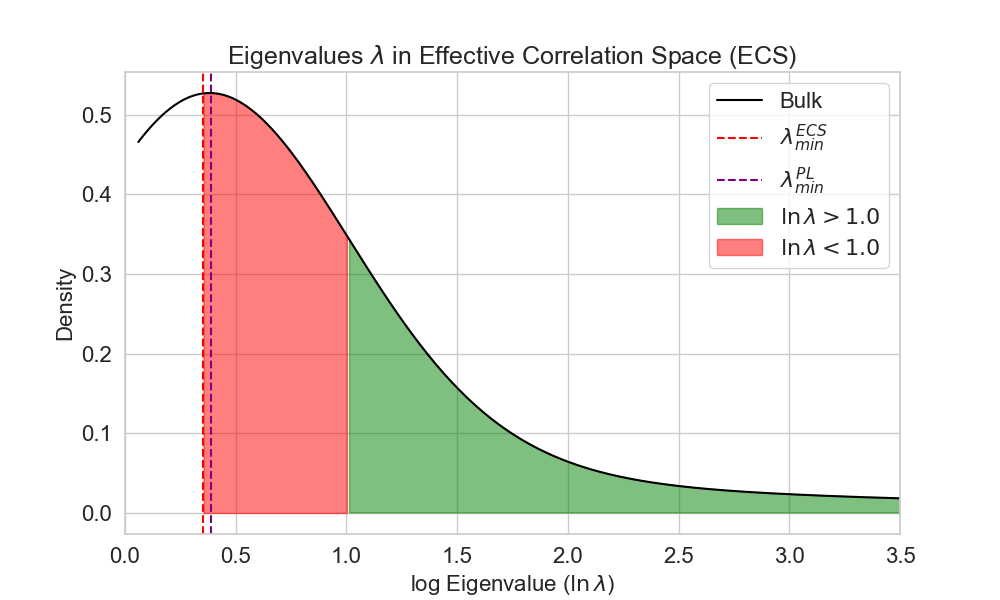
\includegraphics[width=10cm]{./img/ECS_space.png}
  \caption{The image depicts a typical
    \EmpiricalSpectralDensity (ESD) of a layer correlation matrix $\XMAT$, with \WW Power-Law (PL) exponent
    $\alpha=2.0$.%, normalized such that $\Trace{\XMAT}=\Vert\WMAT\Vert^{2}_{F}=N$.
    The green and red shaded regions depict
    eigenvalues $\lambda$ in the \EffectiveCorrelationSpace (\ECS) of $\XECS$, defined by $\lambda>\lambda_{min}^{ECS}$.
    The x-axis displays the eigenvalues on the log scale, $\ln\lambda$.
    The vertical red line is at the start of the PL tail  $(\lambda_{min}^{PL})$.
    The purple, vertical line is at the start of the~\ECS tail  $(\lambda_{min}^{ECS})$.
    The green shaded region depicts those eigenvalues where $\ln\lambda>1.0$,
    whereas the red shaded region depicts those eigenvalues where $\ln\lambda<1.0$.
    The~\ECS is defined such that the volume-preserving~\TRACELOG condition is best satisfied, i.e $\sum\ln\lambda= 0$ for $\lambda\ge\lambda_{min}^{ECS}$.
    }
  \end{center}
  \label{fig:ECS_space}
\end{figure}

Because the \Teacher ESD is most likely MHT and PL, 
if we choose $\lambda_{min}^{ECS}$ too small, and the tail extends too far into the bulk region of the ESD,
then for all practical purposes $\Det{\XECS}\ll 1$.
On the other hand, if we choose $\lambda_{min}^{ECS}$ too large,
then we only capture very large eigenvalues, and for all practical purposes $\Det{\XECS} \gg 1$.
Therefore, if we set the scale of $\XECS$ appropriately, we can choose a $\lambda_{min}^{ECS}$ such that $\Det{\XECS}=1$.
In this case, by choosing $\LambdaECSmin$ appropriately, we can estimate the expected value of
$\langle\Det{\AMATM}\rangle$  with an empirical point estimate over the \Teacher Correlation matrix, which is unity.
\begin{equation}
\label{eqn:detX}
\vert\det\XECS\vert \simeq 1 ; \quad \Trace{ \ln\XECS } = \ln\vert\det\XECS\vert \simeq 0  .
\end{equation} 

This expression can now be used in a practical calculation to define a low-rank subspace that both allows us to evaluate the HCIZ integral,
and to identify, in principle, generalizing components of the layer.
We also refer to \EQN~\ref{eqn:detX} as the \TRACELOG condition, which is technically its empirical form.
\michaeladdressed{Note by abuse of terminology.}
For example, Figure~\ref{fig:ECS_space} depicts the eigenvalues in the~\ECS for a \Typical ESD with PL $\alpha=2.0$,
(normalized such that $\Trace{\XMAT}=\Vert\WMAT\Vert_{F}=N$).
Notice that the start of the PL tail, $(\lambda_{min}^{PL})$, is very close to the start of the~\ECS tail. $(\LambdaECSmin)$,
i.e. $\Delta \lambda_{min}:=\LambdaECSmin-\LambdaPLmin\approx 0$.
Also, notice that while there are many large eigenvalues, $\ln\lambda>1.0$, there are numerous small eigenvalues as well,
$\ln\lambda<1.0$, such that the $\sum\ln\lambda\approx 0$ for $\lambda\ge\lambda_{min}^{ECS}$. In other words, the red and green shaded areas have the same measure.
Additional plots like Figure~\ref{fig:ECS_space}, generated with \WW,  can be found in Section~\ref{sxn:empirical},
in Figure~\ref{fig:mlp3-detx-gap}
as well as plots of $\Delta \lambda_{min}$ vs. the \WW PL $\alpha$ for several real-world examples,
in Figures~\ref{fig:CV_ESD_trends} and ~\ref{fig:LLM_ESD_trends}.


%\subsection{Evaluating the HCIZ Integral in the Large-$N$ Limit}
\subsection{Evaluating the Layer Quality \texorpdfstring{$(\Q)$}{Q} in the Large-\texorpdfstring{$N$}{N} Limit}
\label{sxn:matgen_evaluation_hciz}

%%%Here, we model the matrix-generalized Average ST \Quality (Squared)
%%%$\QT$ of an HCIZ integral, and in the large-$N$ limit. 
%%%\michael{Why change notation below?  I sort of like it but sort of dont.}
%%%We can write the generating function $\IZG$ (for the Total Average \Quality Squared $\mathcal{Q}^{2}$)
%%%in \BraKet notation as
%%%\begin{align}
%%%  \label{eqn:IZG_hciz}
%%%  \IZG := & \frac{1}{N}\left\langle     \exp ( N\beta \Trace{\tfrac{1}{N} \TMAT^{T}\AECS_{2}\TMAT })\right\rangle_{\AECS} 
%%%\end{align}
%%%or explicitly as an integral as
%%%\begin{align}
%%%  \label{eqn:IZG_integral}
%%% \IZG  := & \frac{1}{N}\int d\mu(\AECS) \exp ( N\beta \Trace{\tfrac{1}{N} \TMAT^{T}\AECS_{2}\TMAT })
%%%  \end{align}
%%%or, in Tanakas notation,
%%%\begin{align}
%%%  \label{eqn:IZG_tanaka}
%%% \IZG  := & \frac{1}{N}\mathbb{E}_{\AECS}\left[ \exp ( N\beta \Trace{\tfrac{1}{N} \TMAT^{T}\AECS_{2}\TMAT })\right]
%%%\end{align}
%%%where 
%%%$\langle\cdots\rangle_{A}=\int\cdots d\mu(A)=\mathbb{E}_{A}[\cdots]$
%%%are equivalent notation denoting the expected value (or average) over all \Student Correlation Matrices $\AECS$ spaning the~\ECS,
%%%$\AECS_{2}$ is a (random) $N\times N$ square (correlation) matrix, and
%%%$\TMAT$ is a (non-random) \Teacher $N\times M$ rectangular (weight) matrix.
%%%That is, $\TMAT$ the actual layer weight matrix $\TMAT=\tilde{\WMAT}$ of the model we wish to study
%%%(but also only in the span of the~\ECS).
%%%Notice also that, here,  $\beta$ is the inverse-Temperature and not the simple constant $1$ or $2$ as in \cite{Tanaka}.
%%%
%%%\nred{REPEATED AGAIN}
To generate the Average \Quality, $\QT$, we first take the large-$N$ limit of $\IZG$
\begin{equation}
  \label{eqn:IZG_limit}
  %  \IZGINF := \lim_{N\gg 1}\IZG = \lim_{N\gg 1}\ln\; \mathbb{E}_{\AECS}\left[\exp N\beta\left( \tfrac{1}{N}\Trace{ \TMAT^{\top}\AECSN\TMAT } \right)\right] ,
\IZGINF := \lim_{N \gg 1} \IZG 
= \lim_{N \gg 1}   \red{\tfrac{1}{N}}
\ln \; 
  \Expected[\AECS]{ 
    \exp\,
      N \beta \Trace{\tfrac{1}{N}\TMAT^{\top}\,\AECSN\,\TMAT}
  } 
\end{equation}
and then take the appropriate partial derivative,
analogously to how we did for $\AVGSTGE$; see Section~\ref{sxn:quality} for more details.
This gives (as in \EQN~\ref{eqn:QT_def})
\begin{align}
\label{eqn:IZG_generate_Q2}
\QT &:= \frac{1}{\beta}\frac{\partial }{\partial \ND}\IZGINF  \\ 
&\underset{\text{high-}T}{\approx}
\frac{1}{\ND}\frac{\partial }{\partial \beta}\IZGINF 
\end{align}
Notice that since we are at high-Temperature, it doesn't matter which partial derivative we take,
and we expect both results to be yield the same expression.

This HCIZ integral in \EQN~\ref{eqn:IZG_limit} can be evaluated
(i.e in the large-$N$ limit) using a result by Tanaka ---provided
the matrix $\AECSN$ is low rank, which holds when the \TRACELOG condition is satisfied.
Thus, moving forward, we will assume an
\EffectiveCorrelationSpace (\ECS) of rank $\MECS$, where $\LambdaECSmin$ is the $M^{th}$-largest eigenvalue of $\XECS$,
and defines the start of the~\ECS (and whatever branch-cut is necessary to integrate $R(z)$).

Tanaka's result for the~\ECS can be expressed as:
\begin{equation}
  \label{eqn:tanaka_result}
  \underset{N\gg 1}{\lim}\frac{1}{N}\ln
\Expected[\AECS]{\exp\left(\ND\beta \Trace{\TMAT^{\top}\AECSN\TMAT}\right)}
  =\ND\beta\sum\limits_{i=1}^{\MECS}\;\GNECSI,
\end{equation}
where the sum now only includes the eigenvalues of $\XECS$ (in the~\ECS), $\beta=\tfrac{1}{T}$
is the Inverse-Temperature, and $\LambdaECS$ is an eigenvalue of $\XECS$, the Teacher
Correlation matrix projected into the \ECS space.
$\AECSN$ is the $N \times N$ form of the \Student Correlation matrix,
with $N-M$ non-zero eigenvalues, and $\TMAT$ is the $N\times M$ \Teacher  weight matrix
(also effectively projected into the \ECS, i.e. $\TMAT=\TECS$ here).
$\GNI$ is the \GEN, defined below.
\footnote{We use the notation $\Expected[\AECS]{\cdots}$ for expected value and placed $\tfrac{1}{N}$ on the L.H.S.
to help the reader compare this to the original expressions in~\cite{Tanaka2007, Tanaka2008}.
Also,  in \cite{Tanaka2007, Tanaka2008},$\beta=1|2$, but, in fact, if one inserts $-\beta$ as an inverse temperature into the final expression, it simply factors out.}
This gives
\begin{equation}
\label{eqn:tanaka_result2}
\IZGINF = \ND\beta\sum\limits_{i=1}^{\MECS}\;\GNECSI,
\end{equation}
\michaeladdressed{State this in a self contained way, with rank assumptions, etc.}


This gives a final expression for the Average \LayerQuality (Squared) $\QT$ as
\begin{equation}
\label{eqn:Q2_result}
\QT = \sum\limits_{i=1}^{\MECS}\;\GNECSI,
\end{equation}
Note that $\QT$ is independent of $N$ and $\beta$,
and, indeed, \EQN~\ref{eqn:IZG_generate_Q2} is an equality.

The average \Quality (squared) can be expressed as a sum over
\GeneratingFunctions $\GN$, which depend only the statistical properties of the
actual \Teacher Correlation  matrix  $\XECS$ (projected into the~\ECS).
Each term in the sum, $\GNECSI$, takes the form
\begin{equation}
\label{eqn:generating_function_A}
 \GN:=\int\limits_{0}^{\lambda}R_{\AMAT}(z)dz \xrightarrow{\text{\ECS}}\int\limits_{\LambdaECSmin}^{\lambda}R_{\AECS}(z)dz
\end{equation}
where $R_{\AECS}(\LambdaECS)$ is the \RTransform from RMT,
and $\LambdaECSmin$ is the lower bound of the~\ECS spectrum.
Importantly, the \RTransform for a Heavy-Tailed ESD may have a branchcut at or near the
start of the~\ECS (as explained in Section~\ref{sxn:r_transforms}), so restricting the integrand
to start at $\LambdaECSmin$ is critical.

\charles{
  should we call $\GN$ a Generating Functiton or maybe a Norm \GeneratingFunction because the simplest result is something like a  Trace Norm ?
 }

\charles{removed section below for space reasons; see tex file}
%The \RTransform is like an inverse Greens function and is also a Cumulant generating function.
%\michael{Still to fix this par.}
%Specifically, the $R$-transform arises in RMT in the following way. 
%gWe can define the Greens function $\mathcal{G}_{A}(z)$ for any square, positive-definite matrix $\AECS$ as the Steiljes Transform of the ESD $\rho_{A}(\lambda)$.
%\michael{Clarify.}
%Following Zee~\cite{Zee:Blue}, we call $\mathcal{B}(z)$ the \BlueFunction, which is the functional inverse of $g(\AECS)$
%For example, if $\mathcal{G}_{A}(z)=XXX$ then  $\mathcal{B}(z)=YYY $.
%We can then define the $R$-Transform $R(z)$ in terms of $\mathcal{B}(z)$ as XXX.  
%\michael{What does that mean?}
%\charles{RMT has its own Cumulant generating function}

%\michael{Either modularize thias a remark, or lets give an explicit equation that we need to call for our subsequent derivation, or for others to follow up on our derivation.}
%The $R$-tramsform is commonly referred to as the Cumulant Generating Fucntion for RMT.
%However, it also has another interpretation, which is relevant here. 
%Obviously, the R-tramsform of a matrix $\AECS$ can be thought of as a modified functional inverse of the Greens function for $\AECS$,
%
%More importantly, however, if one considers the $R$-transform of the sum of two matrics $\AECS_{2}+\AECS_{2}$, then the resulting expression represents a kind of single-particle Greens function for the interacting matrices~\cite{Zee:Blue}.
%
%Most importantly, we know the $R$-transform for an HT random matrix with a PL ESD (see \EQN~\ref{eqn:R_PL}, below).

\michael{@charles: if I understand things, the following (until the end of the section) is a big shift; we are going from doing Tanaka, to justifying why we use the empirical data; we should highlight it more clearly.}
\charles{@michael: thats true}

Since we expect the best Student matrices to resemble the actual \Teacher matrices, we expect the \Student correlation matrix $\AECS$ to have similar spectral properties to our actual empirical correlation matrices $\XECS$.
That is, from the perspective of \HTSR theory and the classification into \PhasesOfTraining~\cite{MM18_TR_JMLRversion}, we expect all the $\AECS$ to be in the same phase as $\XECS$ (and, in addition, to have the same PL exponent value).   That is, 
\\
\\
\emph{We expect the \RTransform of $\AECS$ to have the same functional form as the $R$-transform of $\XECS$.}
\\
\\
If our (\Teacher) NN weight matrix exhibits a HT PL, then the tail the ESD ($\rho_{tail}(\lambda)$) of the \Student and \Teacher will both take the limiting form of a PL, with the same empirical variance $\sigma^{2}$ and (critically) the same PL exponent $\alpha$:
\begin{equation}
\label{eqn:R_PL}
  \rho_{tail}[\AECS](\lambda)\sim\rho_{tail}[\XECS](\lambda)\sim\lambda^{-\alpha}.
\end{equation}

Up until this point, our derivation of $\QT$ only depends on the \TRACELOG condition, irrespective of the exact functional form of $R(z)$,
therefore the \SETOL approach tested by examining how well the \TRACELOG condition holds for the layers in very well performing models.
We do this in Section~\ref{sxn:empirical-trace_log}.






\subsection{Modeling the R-Transform}
\label{sxn:r_transforms}

\charles{NOTE: There is some subtly here to deal woith because of the branch cuts expected in $R(z)$
  We can derive \ALPHAHAT from the R-Transform, but its a bit lengthy.
  I will also work out the R transform for the truncated power law for $\alpha=2$ and maybe $3,4$ and explain}

In this section, we explain how to select the \RTransform $R(z)$ and evaluate the~\GEN~$\GN$ under different modeling assumptions.
To apply \SETOL, the model satisfy the \TRACELOG condition--which occurs during the case of  \IdealLearning.
For most cases of NN models, the ESD are HT; and this, in practice, one usually would select $R(x)$ that reflects this. 
We analyze several cases, noting their applicability to real-world scenarios.
Most importantly,  we derive expressions that resemble the~\WW~\ALPHAHAT metric, at least formally valid
for the case $\alpha\approx 2$.

\michaeladdressed{We should note here that for some or all of these derivations we obtain results only when we have \IdealLearning.}


\subsubsection{Elementary Random Matrix Theory}
\label{sxn:r_transforms:elementary_rmt}

We beging with some useful notions definitions from \RandomMatrixTheory.
%
Using the ESD $\rho(\lambda)$, defined as
\begin{equation}
\label{eqn:rgo}
\rho(\lambda):=\frac{1}{N}\sum_{i}\delta(\lambda-\lambda_{i})  ,
\end{equation}
%
we can express the \emph{\GreensFunction} (or \emph{\Cauchy}-Stieltjes transform) by%
\footnote{Please notice our naming and sign convention in \EQN~\ref{eqn:Cz}.
\michaeladdressed{Which? Or is this the def here?}
\charles{@michael: it a sign convention. Read forward}
Some authors equate the \GreensFunction $G(z)$ with
the \Cauchy-Stieltjes transform, whereas we define $C(z)=-G(z)$.}
\begin{equation}
\label{eqn:Gz}
G(z):=\int \mathrm{d}\lambda \frac{\rho(\lambda)}{z-\lambda} .
\end{equation}
%
From $G(z)$, we can recover the ESD, $\rho(\lambda)$, using the inversion relation
\begin{equation}
\label{eqn:GzInverse}
\rho(\lambda)=\lim_{\epsilon\rightarrow 0+}\frac{1}{\pi}\mathrm{IM}(C(\lambda+i\epsilon))  ,
\end{equation}
where $\mathrm{IM}$ is the imaginary part of $G(z)$, and where the $\lim_{\epsilon\rightarrow 0+}$ means to take the limit approaching from the upper half of the complex plane.
%
The \RTransform, $R(z)$, can be defined using the Blue function $B(z)$ 
\begin{equation}
\label{eqn:Rz}
R(z):=B(z)-\frac{1}{z}  ,
\end{equation}
where the Blue function $B(z)$~\cite{Zee1996} is the functional inverse of the Greens Function $G(z)$,% 
\footnote{The Blue function was first introduced by Zee~\cite{Zee1996} to model, among other things, spectral broadening in quantum systems.
Briefly, given a deterministic Hamiltonian matrix $\mathbf{H}_{0}$, with eigenvalues $\lambda^{0}_{i}$,
one can model the spectral broadening of $\lambda^{0}_{i}$ by adding a random matrix $\mathbf{H}_{1}$ to $\mathbf{H}_{0}$:
$\mathbf{H}=\mathbf{H}_{0}+\mathbf{H}_{1}$.  
The resulting eigenvalues of $\mathbf{H}$ now contain some level of randomness, $\sigma$, i.e., $\lambda=\lambda^{0}+\sigma$.  
To model the ESD of $\mathbf{H}$, one then specifies the invididual \RTransforms for $\mathbf{H}_{0}$ and $\mathbf{H}_{1}$; the full ESD of $\mathbf{H}$
can then be reconstructed by adding the two \RTransforms together $R(z)=R_{0}(z)+R_{1}(z)$.
Zee also notes that $R(z)$  is the same as the self-energy $\Sigma(z)$ from quantum many body theory~\cite{Zee1996}.}
satisfying 
\begin{equation}
\label{eqn:GzRelation}
B[G(z)]=z  .
\end{equation}
By specifying the $R(z)$ transform, we specify the complete ESD, $\rho(\lambda)$.
Here, we are actually only interested in the tail of $\rho(\lambda)$.
%and we can accept errors in $R(z)$ that describe the bulk region inaccurately or improperly. 
That is, we can given $R(z)=R(z)_{tail}+R(z)_{bulk}$, we only need $R(z)\approx R(z)_{tail}$.
\michaeladdressed{Good point to make here, but we need to make clear that our bulk/tails are not their bulk/tails.}
\charles{@michael: who is 'they' ?  }

\charles{Describe $R(z)$ is a power series, and how we take $\int dz R(z)$ and why we restirct the integral, contours, etc}



\subsubsection{Known \RTransforms and Analytic (Formal) Models}
\label{sxn:r_transforms:known_r_transforms}

There only a few known analytic results for the explicit \RTransform $R(z)$.
Below, we review some of them, explaining what ESD they correspond to,
and what the resulting \GEN~$G(\lambda)$ would be if applied
as a model $R(x)$ in the \SETOL approach.

See Table~\ref{tab:known_r_transforms}.

\nred{Note: removed \emph{Multiplicative-Wishart} }
\begin{table}[h!]
  \centering
  \renewcommand{\arraystretch}{1.25} % Increase line spacing in table
\begin{tabular}{|c|c|c|}
  \hline
  Model & \HTSR Universality class & \RTransform $R(z)$\\  \hline
  \hline
  Discrete & Spikes & $\tfrac{1}{\MECS}\sum_{i=1}^{\MECS}\lambda_{i}$   \\ \hline
  \hline
  Wishart Models & &\\ \hline
%  Multiplicative-Wishart & HT/VHT& $\dfrac{\epsilon\phi z^2}{2 - \epsilon\phi^2 z^2}$ \\  \hline
  \InverseWishart & HT/VHT &  $\dfrac{\kappa-\sqrt{\kappa(\kappa-2z)}}{z}$  \\  \hline
   \hline
  Levy \Wigner &   & \\  \hline
  General  $(\alpha_{l}\ne 1)$ & VHT/HT  & $a+bz^{\alpha_{l}-1}$ \\  \hline
  \Cauchy $\alpha_{l}=2, \beta=0$ & $\alpha=2$ & $a - i\gamma$ \\  \hline
\end{tabular}
\caption{Known \RTransforms for different matrix models.
%  The \emph{Multiplicative-Wishart} model has two real, non-zero parameters, $\epsilon$ and $\phi$; for more details, see \cite{Pennington2017}.
  For the \emph{\InverseWishart}, as given by Bun~\cite{BunThesis}, $\kappa=\frac{1}{2}(Q-1)$ where, $q=\frac{1}{Q}=\frac{M}{N}\le 1$.
  The \emph{\LevyWigner} model describes \Wigner-like Square Random Matrices
  (as opposed to Wishart-like or Correlation Matrices), where the elements are drawn from a Levy-Stable distribution.
  The Levy-Stable $R(z)$ is parameterized by a (real) shift parameter $a$,
  a complex phase factor $b$ (that depends on 3 real parameters  $\alpha_{l}, \beta$, and $\gamma$),
  and, importantly,  a PL-like tail exponent $\alpha_{l}\in (0,2)$;
  For more details, the text, see~\cite{BJNx01_TR,BJNx06_TR,BJ09_TR}.
  \red{For our modeling purposes here, we make the association $\alpha_{l}\sim\alpha/2-2$. maybe not?}
  (Also, for simplicity, we assume the variance $\sigma=1$ for all models above, where appropriate.)
  \michaeladdressed{Is that assumption just for this table.}
  \charles{@michael: yes}
}  
\label{tab:known_r_transforms}
\end{table}

\charles{Discuss the Table briefly, and then each model in its own subsubsection.
We can create plots to show how these models can treat heavy tails, and explain the parameter fitting
}
\michael{We have five rows in the table but three subsubsxns below. How many do we have? Maybe make each a par rather than a subsubsxn.}
\charles{@michael: this is low priority, can revisit later}

\subsubsection{Discrete Model: Spikes}

Here, we consider modeling the HT tail ESD, $\rho_{tail}(\lambda)$, as a collection
of discrete spikes $\lambda_{spike}$, 
where $\lambda_{spike}\ge \LambdaECSmin$.
Here, \RTransform for the \ECS is sum of Dirac delta functions  (as opposed to using
the Inverse-Wishart (IW) or other model $R(z)$.)
This lets us compute the \LayerQuality $\Q$ in closed form in term of the Teacher weight matrix
$\TMAT=\WMAT$.

\michaeladdressed{What is the meaning of the thing we derive if the \TRACELOG condition doesn't hold? Do we have any control on it?  And what do you mean it doesn't hold? }
Let the tail of the ESD have $\MECS = M^{tail}$ eigenvalues that define the \ECS, i.e.,  
\begin{equation}
\label{eqn:spikes_model_0}
\rho_{tail}(\lambda)=\sum_{i=1}^{\MECS}\delta(\lambda-\lambda_{i}) .
\end{equation}
\michaeladdressed{Let's sync, since I don't know what that phrase means in this context, and I want to make sure we didn't introduce a confusion above.}
\charles{@michael: seriously?!  We have discussed this multiple times.  We dicussed it at dinner in New Orleans.}
The \GreensFunction $G(z)$ is then
\begin{equation}
\label{eqn:spikes_model_1}
G(z) = \int d\lambda \dfrac{ \rho_{tail}(\lambda) }{z - \lambda} =
\sum_{i} \int d\lambda \dfrac{\delta(\lambda-\lambda_{i}) }{z - \lambda} =
\sum_{i} \dfrac{1}{z-\lambda_{i}}  ,
\end{equation}
and the Blue function for each invividual term $i$ is $\frac{1}{z-\lambda_{i}}$, i.e., $B(z)=\lambda_{i}+\frac{1}{z}$. 
Now, using the additive property of the \RTransform, we can express the total $R(z)$ as the sum of the \RTransforms for the individual terms $i$, giving
\begin{equation}
\label{eqn:spikes_model_2}
R(z) =\sum_{i}\left(\lambda_{i}+ \dfrac{1}{z}\right) - \dfrac{1}{z}=
\sum_{i}\lambda_{i}  .
\end{equation}
This gives the \GEN~$\GN$ as
\begin{align}
\label{eqn:spikes_model_3} 
\GN 
&= \int_{\LambdaECSmin}^{\lambda}\sum_{i}\lambda_{i} d\lambda \\ \nonumber
&= \sum_{i}\lambda_{i} \int_{\LambdaECSmin}^{\lambda} 1 d\lambda \\ \nonumber
&= \left(\sum_{i}\lambda_{i}\right)\left(\lambda-\LambdaECSmin\right)
\end{align}
Seeing that $\LambdaECSmin$ is usually quite small, we make the approximation
\begin{align}
\GN  \approx \left(\sum_{i}\lambda_{i}\right)\left(\lambda\right)  ,
\end{align}
which gives the \QualitySquared approximately as
\begin{align}
  \label{eqn:spikes_model_4}
  \QT = \sum_{i}\GNI 
 \approx\left(\sum_{i}\lambda_{i}\right)^{2}  .
\end{align}
We now see that we can define $\Q:=\sqrt{\QT}=\sum_{i}\lambda_{i}$ is what we call a Tail Norm.

\nred{CHECK FOR ERRORS PLEASE; Also ?  not really a Trace norm since this is defined over singlular values ?}
\michael{MM TO DO: connect to trace norm; the singular value thing should be okay.}
\charles{@michael: then do it}


%The Multiplicative-Wishart (MW) model  has two real, adjustable parameters $\epsilon,\phi$.
%It treates $\mathbf{X}$ as resulting from product of random matrices, and is good for modeling an ESD with a very heavy tail.
%It has been used previously to model the heavy tail of the Hessian matrix in NNs\cite{Pennington2017}
%This model would work better for fitting HT ESDs that decay slower than a TPL.  We will not consider
%this model further here and leave this for future work.

%We will work out  the full details, going from $\rho(\lambda)\rightarrow G(z)\rightarrow R(z)\rightarrow \QT$


\subsubsection{Inverse-Wishart Model of \IdealLearning}

Here, we consider the \InverseWishart (IW) model.
The IW model treats the ESD of $\mathbf{X}^{-1}$ when the ESD of $\mathbf{X}$ itself is MP.
As a parametiric model, it can be quite effective at treating VHT and HT (or \FatTailed) ESDs when the far tail decays very rapidly, like a TPL, and/or for $\alpha\le 4$.
To do this, one simply considers the parameters $\kappa$ as an adjustable paremeter.
\michaeladdressed{Give a functional form, with $\kappa$ appearing.}
\charles{@michael: do it yourself or don't suggest it}
%
It is an excellent model for the ESD when $\alpha=2.0$ (and $Q=2$).
Using this model, we can derive an expression for the \HTSR \ALPHAHAT \LayerQuality metric,
$\ALPHAHATEQN :=\ALPHAHATLONG)$ as a leading order term in the final expression for $\log_{10}\QT$.

This model 


\begin{figure}[h]
    \centering
    \subfigure[IW Distribution, $\kappa=0.25$]{ 
      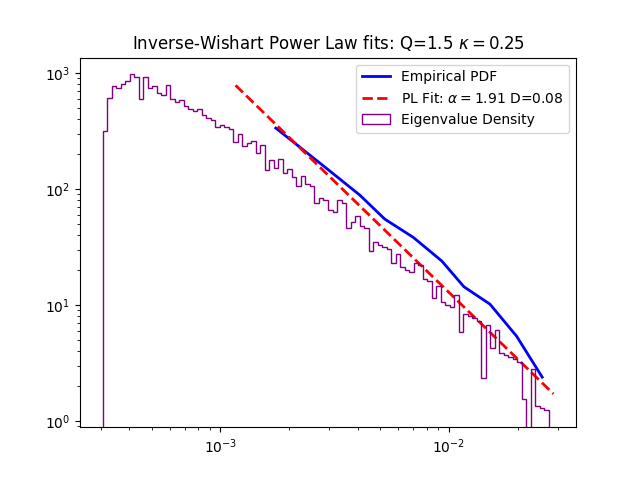
\includegraphics[width=5cm]{./img/IWplotQ1.5.png}
      \label{fig:IWplotQ15}                                                                                                      
    }                               
      \subfigure[IW Distribution, $\kappa=1.25$]{ 
      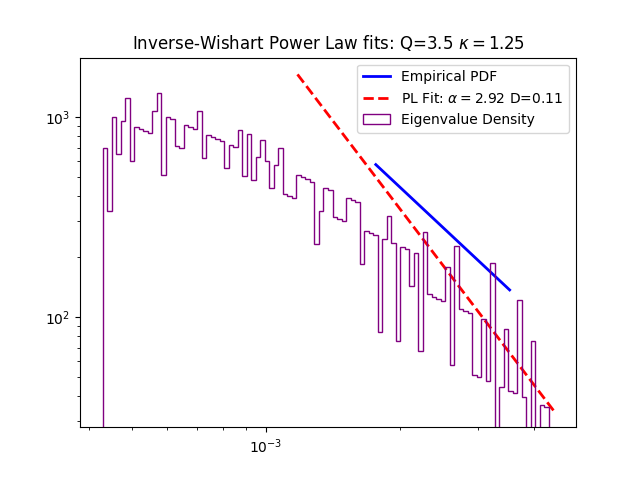
\includegraphics[width=5cm]{./img/IWplotQ3.5.png}
      \label{fig:IWplotQ35}                                                                                                      
      }
      \caption{Example Inverse-Wishart (IW) distributions for $\kappa=0.25$ and $\kappa=1.25$,  along with Power Law (PL) fits of the generated distribution. Plots on Log-Log scale.}
  \label{fig:IWplots}                                                                                                      
\end{figure}   

In Figure~\ref{fig:IWplots}, we fit some \Typical layer ESDs to an IW distribution.
When $\kappa=0.25$, the fitted $\alpha=1.91$, and the fit is a reasonably accurate model of the underlying Power Law
distribution and the ~\WW PL fit.
For  $\kappa=1.25$, the fitted $\alpha=2.92$ is larger, but the fit is not as good as a
model. Generally speaking, $\alpha$ scales with $\kappa$, but the  free cumulants scale inversely with $\kappa$.
So smaller $\alpha$ will give larger free cumulants and therefore a larger $\QT$.
Importantly, as seen in Figure~\ref{fig:IWplotQ15}, for $\alpha=\simeq 2.0$, the IW model (with $\kappa=0.25$)
is an effective simple model to illustrate the \SETOL case of \IdealLearning.
\michaeladdressed{Maybe this par and fig elsewhere; or at end of subsubsxn.}
\charles{@michael: low priority; can revisit}

\begin{figure}[t]
    \centering
    \subfigure[IW $R(z)$, real $z$.]{
        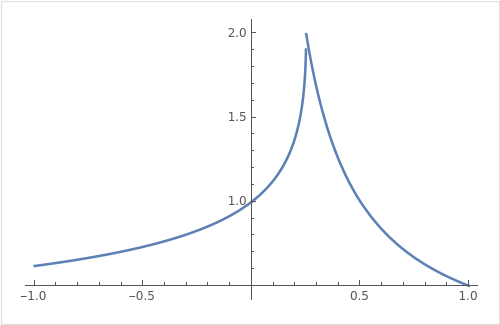
\includegraphics[width=4cm]{./img/R.png}
        \label{fig:IW_R}
    }
    \subfigure[Branch cut at $z=\kappa/2$]{
        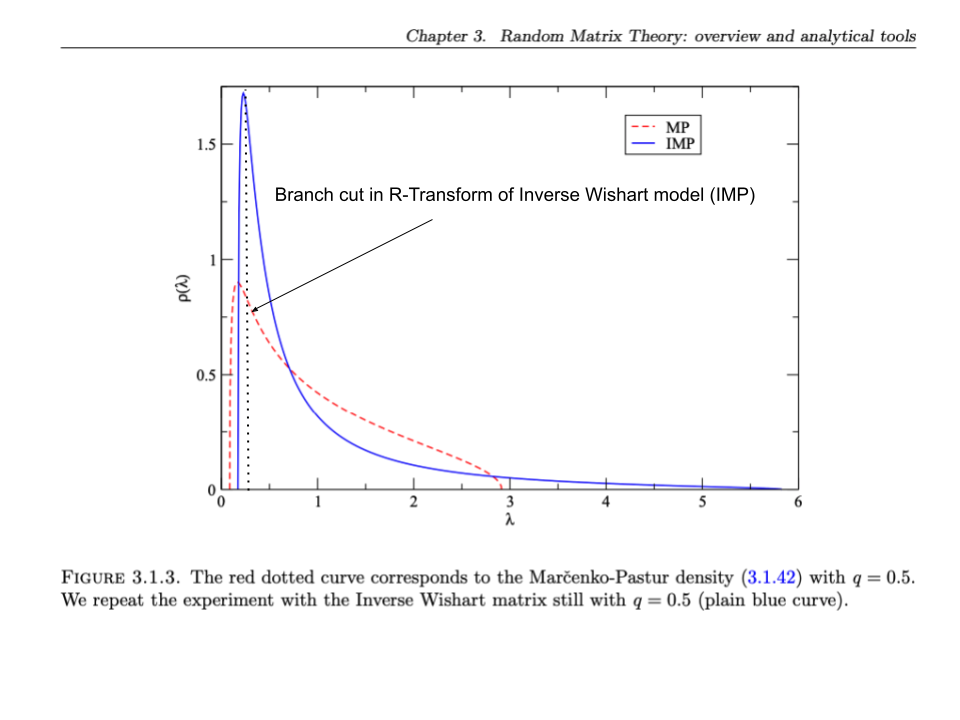
\includegraphics[width=4cm]{./img/branch-cut.png}
        \label{fig:IW_branch_cut}
    }
    \caption{(a) The function $R(z)$ of the Inverse Wishart model, with a singularity at $z = \kappa/2$. (b) The branch cut in the empirical spectral density, corresponding to the tail for $\kappa = 0.5$.}
    \label{fig:R_branch_cut_combined}
\end{figure}

Lets consider $R(z)$ for the \InverseWishart model, denoted $R(z)[IW]$.
To integrate this function, we require that it be analytic.
At first glance, it may seem that that $R(z)[IW]$ is not analytic because it
has a pole at $z=0$ and because the square-root term $\sqrt{\kappa(\kappa-2z)}$  creates branch
cut at and $z=\kappa/2$ (and $z=\infty$).
Figure~\ref{fig:R_branch_cut_combined} presents this in two ways:
Figure~\ref{fig:IW_R} shows the R-transform $R(z)[IZ]$ for real $z$, highlighting its singular behavior and the location of the branch cut at $z = \kappa/2$; and
Figure~\ref{fig:IW_branch_cut} shows the corresponding branch cut in the ESD of the Inverse Wishart model (for $\kappa = 0.5$).
We select the branch cut starting at $z=\kappa/2$ and ending at $z=\infty$,
which allows us to at least formally defined the integral along the physically meaningful part of the ESD:
\begin{equation}
\label{eqn:IW_model_1} 
\GN[IW] := \int_{\LambdaECSmin}^{\lambda} R(z)[IW] dz  ,
\end{equation}
noting that we expect $\LambdaECSmin\ge\kappa/2$.
\michael{Why do we have this par, if we are using quality squared. I need to understand.}
\charles{@michael: whats the issue ?}

It turns out, however, that due to the branch cut in $R(z)[IW]$,
the function $\GN[IW]$ is not analytic in the domain we need. 
To correct for this, we will instead model the \LayerQualitySquared using the modulus of $\GN[IW]$,
\begin{equation}
\label{eqn:IW_model_1} 
|\GN[IW]| := \sqrt{\GN[IW]^{*}\GN[IW]}
\end{equation}
where $\GN[IW]^{*}$ is the complex conjugate of $\GN[IW]$.
This is somewhat involved, so we present the full calculation in Appendix~\ref{sxn:IW}
\michael{MM TO DO: Go through.}
\michael{Are we going to mention the result here since we will use it?}


Figure~\ref{fig:InverseWishartGx} plots $|\GN[IW]|$ on Lin-lin and Log-log plots, on the range $\lambda\in(0.25, 100)$, and fits the it to a PL. 
The fit follows the general trend of the function, but it is not terribly accurate.
Still, from this plot, we can see that the \LayerQualitySquared has the same general trend as $\ALPHAHAT$ and/or a Shatten Norm.

\begin{figure}[t]
  \centering
  \subfigure[$|\GN\lbrack IW\rbrack|$ Lin-lin plot and PL fit]{
    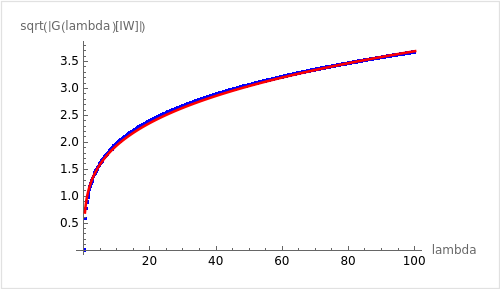
\includegraphics[width=0.45\textwidth]{./img/Gx.png}
        \label{fig:GxPlot}
    }
    \subfigure[$|\GN\lbrack IW\rbrack|$ Log-log plot and PL fit]{
        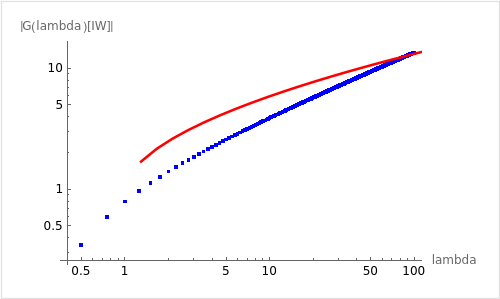
\includegraphics[width=0.45\textwidth]{./img/logGx.png}
        \label{fig:LogLogGxPlot}
    }
    \caption{Behavior of $\GN[IW]$ for the Inverse Wishart (IW) model,
       with a Power Law (PL) fit (red), $|\GN[IW]|\approx 1.138 \lambda^{0.539}$.
      (a)  Lin-lin plot. (b) Log-log plot.
}
    \label{fig:InverseWishartGx}
\end{figure}

%
%\begin{figure}[t]
%    \centering
%    % Subfigure (a): G(x) Plot
%    \subfigure[Inverse Wishart $\GN$]{
%        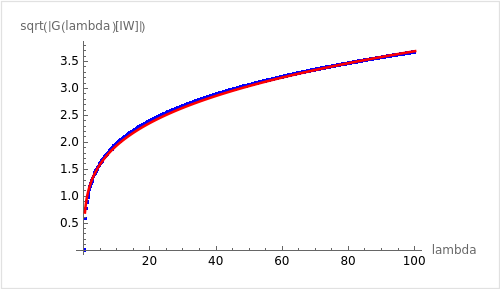
\includegraphics[width=0.45\textwidth]{./img/Gx.png}
%        \label{fig:GxPlot}
%    }
%    % Subfigure (b): Log-log plot and power-law fit
%    \subfigure[Log-log plot and power-law fit]{
%        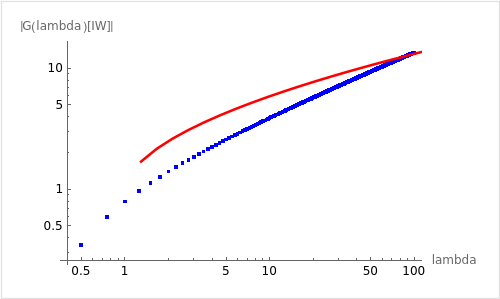
\includegraphics[width=0.45\textwidth]{./img/logGx.png}
%        \label{fig:LogLogGxPlot}
%    }
%    \caption{Behavior of $\GN$ for the Inverse Wishart (IW) model. (a) $\GN$ lin-lin plot. (b) Log-log plot of $\GN$ with a Power Law (PL) fit, $\GN\sim 2.8\lambda^{-3.0}$ }
%    \label{fig:InverseWishartGx}
%\end{figure}
%
%Given an analytic expression for $\GN$ (and $\kappa=0.25$), we can plot the $\GN$ as a function of $\lambda$,
%and then fit this to a Power Law; this is depicted in Figure~\ref{fig:InverseWishartGx}.
%The resulting fit gives $\GN\simeq 2.8\lambda^{3.0}$.
%We can now associate $\ALPHAHAT$ with $\log_{10}\QT$ by keep the leading order term
%$(\lambda_{max}=\LambdaECS_{max}$)
%
%\begin{align}
%  \label{eqn:IW_alphahat}
%  \ALPHAHATEQN:=\ALPHAHATLONG\approx\log_{10}\QT=\log_{10}\sum_{\LambdaECS}\GNI\approx\log_{10}\mathcal{G}(\lambda_{max}\sim (\alpha+1)\log_{10}\lambda_{max}
%\end{align}
%So for $\alpha=2.0$, $\log_{10}\QT\sim (\alpha+1)\log_{10}\lambda_{max}$, which is very close to $\alpha\log_{10}\lambda_{max}$. QED.


\subsubsection{Levy-Wigner Models and the \ALPHAHAT Metric}

Here, we consider Levy-Wigner Models.
We show how to obtain the \WW~\ALPHAHAT metric by modeling the near VHT cases with an approximation to a Levy distribution at $\alpha\approx 2$.  

We do this because the~\ALPHAHAT metric has been developed to adjust for \SCALE anomalies that arise from issues like \CorrelationTraps,
making \ALPHA smaller than expected.
The  \LevyWigner (LW) model treats  $\mathbf{X}$ as if it were a \Wigner matrix (and not actually a correlation  matrix), and the $\alpha$ is different but related to $\alpha$ above in \EQN~\ref{eqn:rhoX}.
The ESD follows a Levy-Stable distribution, where $a$ is a shift parameter, and $b$ is a complex phase factor depending on 2 real factors, $\beta$ and $\gamma$.
Strictly the ESD for an LW model, $\rho_{LW}(\lambda)$, is defined by its characteristic function (i.e., the Fourier Transform of $\rho_{LW}(\lambda)$), but
we can note that the ESD is VHT, $\rho_{LW}(\lambda)\sim\lambda^{-\alpha-1}$, and that when $\alpha_{l}\approx 1$, the ESD resembles a PL HT ESD with $\alpha\approx 2$.

For case of \IdealLearning,  we choose to \emph{model} the \RTransform of our Fat-Tailed HT ESDs as
\begin{equation}
\label{eqn:LW_model_0} 
R(z)[HT] = bz^{\alpha-1},\;\alpha\simeq 2
\end{equation}
where $b$ is an unspecified constant (possibly negative and/or complex).
\michael{We need to clarify. Are we saying that we do PM instead of LW here.}
Notice that when $\alpha\approx 2$, our model is close to the LW model, $R(z)[HT]\approx R(z)[LW]$
(and gives a \Cauchy distribution if we choose $b=a-i\gamma$).

Integrating $R(z)[HT]$, and (as above) taking the approximation $\LambdaECSmin\sim 0$, we obtain (formally)
\begin{equation}
\label{eqn:LW_model_1} 
\GN[HT] = \tfrac{b}{\alpha} \lambda^{\alpha}  .
\end{equation}
%
If we now choose $b=\alpha=2$, then  $\QT$ takes the form of a Shatten Norm (squared)
\begin{equation}
  \label{eqn:LW_model_2}
  \QT = \tfrac{1}{\MECS}\sum_{i}\lambda^{\alpha}  .
\end{equation}
%
Taking the logarithm of $\GN[HT] $, we obtain
\begin{equation}
\label{eqn:LW_model_3} 
\log \GN[HT] =  \log\tfrac{b}{\alpha} +\tfrac{\alpha}\log\lambda
\end{equation}

As with the \InverseWishart (IW) model, we can derive a formal expression for $\ALPHAHAT$ using the LW model.
To do so, let us approxmate $\QT$ by the largest term in the sum over $\GN$, and then let $\lambda=\lambda_{max}$, giving
\begin{equation} 
\label{eqn:LW_model_4} 
\ALPHAHATEQN = \log_{10} \QT \approx  \alpha\log\lambda_{max}   .
\end{equation}
We present this as a formal example, noting that is slightly different from the result for the IW model, Eqn.~\ref{eqn:IW_alphahat}. 
We do not claim this is a valid empirical model, as we have not attempted to fit a real-world ESD to Levy-stable distribtion.  
\michael{Let's sync on the rationale here, since I'm not sure what is being said.}
We leave this to a future study, noting, however, there has been some work doing such fits~\cite{li2024exploring}.

Ideally, we would like to have an rigorous expression for $R(z)$ not just
in the case of \IdealLearning but also for the entire \FatTailed Universality class.
This is non-trivial to obtain and we will attempt this in a future work.
Fow now, we will take a different approach, and evaluate $R(z)$ explicitly using numerical techniques.


\subsection{Computational Random Matrix Analysis}
\label{sxn:comp_rmt}
The \RTransform is the generating function for the \emph{\FreeCumulants} of RMT.
Formally--and if we assume a model without a branch-cut or troublesome poles--
one can define $R(z)$ as a series expansion in $z$,
\begin{equation}
  \label{eqn:Rz_expansion}
  R(z) := \kappa_1 + \kappa_2 z + \kappa_3 z^2 + \ldots 
\end{equation}
where the coefficients $\kappa_{k}$ are the free cumulants, which can be expressed
in terms of the matrix moments $m_{k}$\cite{FreeCumulants}, defined (here) as
\begin{equation}
  \label{eqn:mk_defn}
  m_{k}:=\Trace{\XECS^{k}}=\sum_{i=1}^{\MECS}(\LambdaECS)^{k}
\end{equation}
where $\LambdaECS_{k}$ is the k-th eigenvalue of the effective correlation matrix $\mathbf\XECS$,
which  has been mean-centered and normalized by its standard deviation.

The free cumulants are defined recursively as
\begin{equation}
  \label{eqn:kappa_defn}
  \kappa_k := m_k - \sum_{\text{partitions of } n} \prod_{\text{blocks } B} m_{|B|} 
\end{equation}
\charles{finish explanation}

The first 5 \emph{\Cumulants} are, explicitly,
\begin{align}
  \label{eqn:kappa_defn_2}
  k_1 = m_1 \\ \nonumber
  k_2 = m_2 - m_1^2 \\ \nonumber
  k_3 = m_3 - 3 m_2 m_1 + 2 m_1^3 \\ \nonumber
  k_4 = m_4 - 4 m_3 m_1 - 2 m_2^2 + 10 m_2 m_1^2 - 5 m_1^4 \\ \nonumber 
  k_5 = m_5 - 5 m_4 m_1 + 15 m_3 m_1^2 + 15 m_2^2 m_1 - 35 m_2 m_1^3 - 5 m_3 m_2 + 14 m_1^5
\end{align}

Using these definitions, we can estimate the \LayerQuality matrix $\QT$ for our experimental models
(in Section~\ref{sxn:empirical} by computing  $\GN$ for the effective correlation space
(i.e. the tail of the layer ESD), however it is defined.  That is, we use

\begin{align}
  \label{eqn:G_lambda_series}
\GNI=\kappa_{1}\frac{\LambdaECS}{\MECS}+\frac{\kappa_{2}}{2}\left(\dfrac{\LambdaECS}{\MECS}\right)^{2}+\cdots
\end{align}
Note that we evaluate $\GN$ using eigenvalues normalized with $\tfrac{1}{\MECS}$.
This is implemented implemented in the ~\WW package.
In Section~\Ref{sxn:empirical_comp_r_transforms}, we examine some examples of this approach to computing \LayerQualities directly.


